

%% AAPT Physics Olympiad F=ma Questions
%%----------------------------------------


%% PhysicsOlympiad 2015
%%----------------------------------------


%% PhysicsOlympiad 2000
%%----------------------------------------
\element{aapt}{ %% Olympiad-B4
\begin{question}{olympiad-2000-q19}
    A student makes a tone by blowing across one end of a tube \SI{0.5}{\meter} long that is open at both ends.
    If the speed of sound is \SI{342}{\meter\per\second},
        what will be the frequency of the fundamental note produced?
    \begin{multicols}{3}
    \begin{choices}
        \wrongchoice{\SI{171}{\hertz}}
      \correctchoice{\SI{342}{\hertz}}
        \wrongchoice{\SI{684}{\hertz}}
        \wrongchoice{\SI{1026}{\hertz}}
        \wrongchoice{\SI{1368}{\hertz}}
    \end{choices}
    \end{multicols}
\end{question}
}


%% PhysicsOlympiad 1999
%%----------------------------------------
\element{aapt}{ %% Olympiad-B4
\begin{question}{olympiad-1999-q22}
    A source when at rest in a medium produces waves with a velocity $v$ and a wavelength of $\lambda$.
    If the source is set in motion to the left with a velocity $v_s$,
        what would be the length of the wavelengths produced directly in front of the source?
    \begin{multicols}{2}
    \begin{choices}
      \correctchoice{$\lambda\left(1-\dfrac{v_s}{v}\right)$}
        \wrongchoice{$\lambda\left(1+\dfrac{v_s}{v}\right)$}
        \wrongchoice{$\lambda\left(1+\dfrac{v}{v_s}\right)$}
        \wrongchoice{$\dfrac{\lambda-v}{v-v_s}$}
        \wrongchoice{$\dfrac{\lambda}{v+v_s}$}
    \end{choices}
    \end{multicols}
\end{question}
}


%% PhysicsOlympiad 1996
%%----------------------------------------
\element{aapt}{ %% Olympiad-B4
\begin{question}{olympiad-1996-q19}
    On a day when the velocity of sound in air is $v$,
        a whistle moves with velocity $u$ toward a stationary wall. 
    \begin{center}
    \begin{tikzpicture}
        %% Floor and Wall
        \draw (-7,0) -- (0,0);
        \node[anchor=north,fill,pattern=north east lines,minimum width=7.0cm, minimum height=0.05cm] at (-3.5,0) {};
        \draw[line width=1.5pt] (0,-0.25) -- (0,3);
        %% cart
        \node[draw,anchor=south,minimum width=1.5cm,minimum height=0.5cm] (A) at (-5,0.4) {};
        %% wheels
        \draw (A.south east) ++(180:0.3cm) arc(-270:90:0.2);
        \draw (A.south west) ++(0:0.3cm) arc(-270:90:0.2);
        %% velocity
        \draw[thick,->] (A.east) -- ++(0:1.5) node[pos=0.5,anchor=south] {$u$};
        %% whistle
        \draw[thick] (A.north) ++(0:0.25) ++ (90:0.25) --++(180:0.5) --++(90:1) --++(0:0.5) --++(270:0.2) --++(180:0.2) -- ++(-60:0.4) -- cycle;
        \draw (A.north) -- ++(90:0.25);
    \end{tikzpicture}
    \end{center}
    The whistle emits sound with frequency $f$. 
    What frequency of reflected sound will be heard by an observer traveling along with the whistle?
    \begin{multicols}{3}
    \begin{choices}
        \wrongchoice{$f \dfrac{v-u}{v+u}$}
        \wrongchoice{$f \dfrac{v}{v+u}$}
        \wrongchoice{$f$}
        \wrongchoice{$f \dfrac{v-u}{v-u}$}
      \correctchoice{$f \dfrac{v+u}{v-u}$}
    \end{choices}
    \end{multicols}
\end{question}
}


%% PhysicsOlympiad 1994
%%----------------------------------------
\element{aapt}{ %% Olympiad-B4
\begin{question}{olympiad-1994-q22}
    A source at rest emits waves with wavelength $\lambda$ in a medium with velocity $v$.
    \begin{center}
    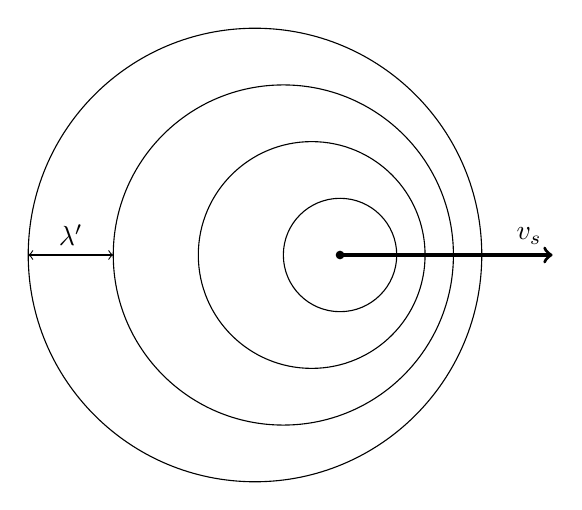
\begin{tikzpicture}[scale=0.9]
        %% Wave Fronts
        \foreach \x in {8,16,24,32} {
            \draw (-0.5 * \x mm,0) circle (\x mm);
        }
        %% Velocity
        \draw[fill] (-4mm,0) circle (1.5pt);
        \draw[very thick,->] (-4mm,0) --++(0:3) node[anchor=south east] {$v_s$};
        %% lambda prime
        \draw[<->] (-48mm,0) -- (-36mm,0) node[pos=0.5,anchor=south] {$\lambda^{\prime}$};
    \end{tikzpicture}
    \end{center}
    If the source moves to the right with velocity $v_s$,
        the distance between adjacent crests $\lambda^{\prime}$ directly behind the source is:
    \begin{multicols}{2}
    \begin{choices}
        \wrongchoice{$\dfrac{\lambda v}{v + v_s}$}
        \wrongchoice{$\dfrac{\lambda v}{v - v_s}$}
        \wrongchoice{$\lambda \left(1 + \dfrac{v}{v_s}\right)$}
      \correctchoice{$\lambda \left(1 + \dfrac{v_s}{v}\right)$}
        \wrongchoice{$\lambda \left(1 - \dfrac{v_s}{v}\right)$}
    \end{choices}
    \end{multicols}
\end{question}
}



\endinput


